%http://www.akxl.net/labs/articles/creating-a-tag-cloud/
%http://www.akxl.net/labs/articles/creating-a-tag-cloud---a-better-approach/
%\listfiles
\documentclass[11pt]{article}
\usepackage{fullpage}
%\usepackage{epsfig}
\usepackage{amssymb}
\usepackage{tocvsec2}
%\usepackage{a4}
\usepackage{fancyhdr}
\usepackage{subfigure}
\usepackage{ifthen}
\usepackage{version}
\usepackage{tocbibind}
\usepackage{makeidx}
%\usepackage{times}
\usepackage{booktabs}
\usepackage[colorlinks=true, pdfstartview=FitV, linkcolor=blue, 
            citecolor=blue, urlcolor=blue]{hyperref}
\usepackage{url}
\raggedbottom
\sloppy

\parindent=0pt
\parskip=5pt

\def\TreeCloud{{\sf TreeCloud }}

%\newcommand\expert[1]{#1}   % expert mode on
\newcommand\expert[1]{}    % expert mode off

%%%%%%%%%%%%%%%%%%%%%%%%%%%%%%%%%%%%%%%%%%%%%%%
\input manualversioninfo.tex
%%%%%%%%%%%%%%%%%%%%%%%%%%%%%%%%%%%%%%%%%%%%%%%

%%%%%%%%%%%%%%%%%%%%%%%%%%%%%%%%%%%%%%%%%%%%%%%
\title{User Manual for \\
\begin{center}
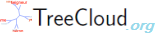
\includegraphics[width=0.3\textwidth]{TreeCloudLogo.png}
\end{center}
version \VERSION ~- \dateversion}
%%%%%%%%%%%%%%%%%%%%%%%%%%%%%%%%%%%%%%%%%%%%%%%

%%%%%%%%%%%%%%%%%%%%%%%%%%%%%%%%%%%%%%%%%%%%%%%

\author{Philippe Gambette}

%%%%%%%%%%%%%%%%%%%%%%%%%%%%%%%%%%%%%%%%%%%%%%%

\makeindex

\input manualdefinitions.tex

\ifx\pdfoutput\undefined
\usepackage[dvips]{graphicx}
\else
\usepackage[pdftex]{graphicx}
\fi

%%%%%%%%%%%%%%%%%%%%%%%%%%%%%%%%%%%%%%%%%%%%%%%
\begin{document}
%%%%%%%%%%%%%%%%%%%%%%%%%%%%%%%%%%%%%%%%%%%%%%%

\maketitle

~\\
~\\

\settocdepth{section}
\tableofcontents

%%%%%%%%%%%%%%%%%%%%%%%%%%%%%%%%%%%%%%%%%%%%%%%
\mysection{Introduction}
%%%%%%%%%%%%%%%%%%%%%%%%%%%%%%%%%%%%%%%%%%%%%%%

\TreeCloud builds a tree cloud visualization of a text, which looks
like a tag cloud where the tags are displayed around a tree to reflect
the semantic distance between the words in the text.

\TreeCloud is a free software licensed under the GPL license.
However, we would greatly appreciate that you follow the instructions
of section~\ref{license} on how to cite the program when you use it.

If you have any problem using \TreeCloud, you can contact
me\footnote{~gambette@lirmm.fr, or \url{http://www.lirmm.fr/~gambette/PersoContactENG.php}}

%% figure %%%%%%%%%%%%%%%%%%%%%%%%%%%%%%%%%%%%%%%%%%%%%%%%%%%%%%%%%%%%%%%%%%%% figure:7views 
\begin{figure}[ht] % b floats figure to bottom, p floats to next page, h = here
\begin{center}
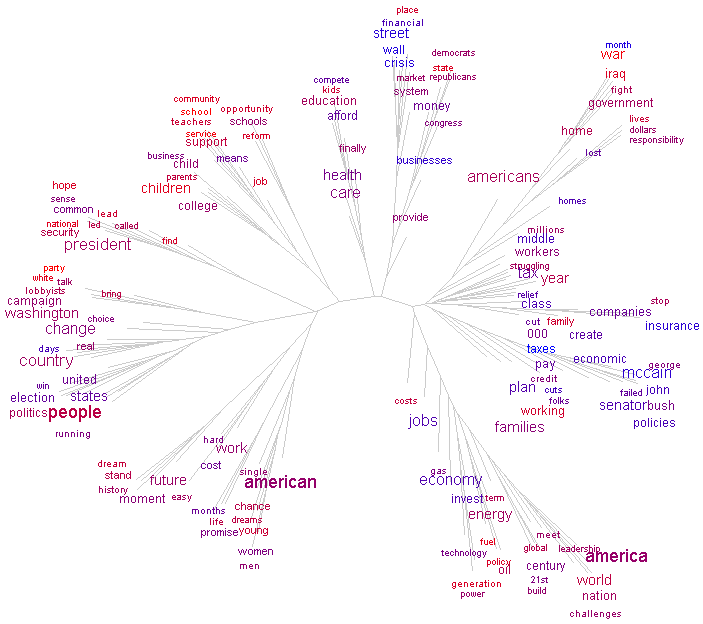
\includegraphics[width=1.0\textwidth]{manualObama2008Campaign.png}
\end{center}
\caption{\small \sffamily Tree cloud of a corpus of Obama's speeches for his 2008 presidential campaign.
\TreeCloud was used with parameters: english stoplist, NJ tree,
\texttt{nbwords=150, window=30, distance=oddsratio, color=chronology}.
}
\label{figure:7views}
\end{figure}
%%%%%%%%%%%%%%%%%%%%%%%%%%%%%%%%%%%%%%%%%%%%%%%%%%%%%%%%%%%%%%%%%%%%%%%%%%%%%%



%%%%%%%%%%%%%%%%%%%%%%%%%%%%%%%%%%%%%%%%%%%%%%%
\mysection{Obtaining and Installing the Program}
%%%%%%%%%%%%%%%%%%%%%%%%%%%%%%%%%%%%%%%%%%%%%%%
Python (version 2.X) should be installed on your system.
If you have OpenOffice,
you may find Python among the OpenOffice files
(for example in \texttt{C:\textbackslash
Program Files\textbackslash
OpenOffice.org 2.4\textbackslash
program\textbackslash
python.bat}).

Then, you should download and install SplitsTree from 
\href{http://www.splitstree.org}
{www.splitstree.org}. You will also need Java to run this program.
Please install SplitsTree in a folder whose path contains
no space. Otherwise, create a link to SplitsTree whose path contains
no space, for example \texttt{C:\textbackslash
TreeCloud\textbackslash
SplitsTree.lnk}

Finally, visit \href{http://www.treecloud.org}
{www.treecloud.org} to download the archive \texttt{Treecloud.zip}
and extract it to a folder where you have writing rights.
Spaces should not appear in the path of this folder.
The two main files of the program
are \texttt{Treecloud.py} and \texttt{TreecloudFunctions.py},
and the Windows program \texttt{Treecloud.exe} is a graphical
user interface which calls \texttt{Treecloud.py} with
the appropriate parameters.

On this website, you can also find stoplists for English, French and German
to remove useless words in the tree cloud (``and'',``of'',``the''\ldots).



%%%%%%%%%%%%%%%%%%%%%%%%%%%%%%%%%%%%%%%%%%%%%%%
\mysection{Using the Program}

\subsection{With the graphical interface on Windows}

When you execute the program \texttt{Treecloud.exe}, the window illustrated
in Figure~\ref{FigGUI} appears.
\begin{figure}[ht] % b floats figure to bottom, p floats to next page, h = here
\begin{center}
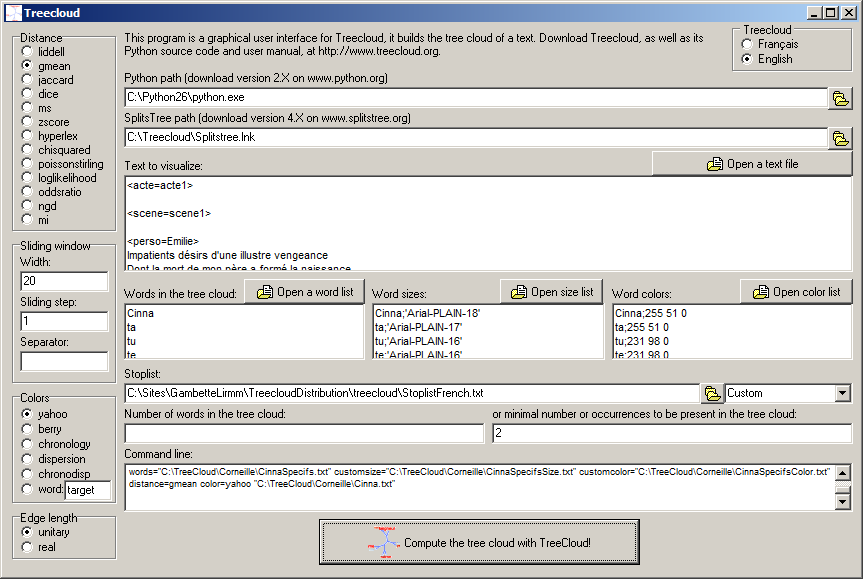
\includegraphics[width=1.0\textwidth]{manualTreecloudGUI.png}
\end{center}
\caption{\small \sffamily Graphical user interface for \TreeCloud on Windows.
}
\label{FigGUI}
\end{figure}
If the color red appears somewhere in the window, it means that there
is a problem you should solve: either Python or SplitsTree was
not found, or there are whitespace in their filenames, or the
stoplist was not found. Correct the problem using the appropriate
buttons.

Once you have set all desired parameters, load a text using the
button labeled \emph{Open a text file}, or paste a text
in the area just below. Use the appropriate stoplist depending
on the text language, and click on \emph{Compute the tree could with TreeCloud!}.
The command line which appears just above this button is then
saved into an MS-Dos command file, \texttt{TreecloudCommand.bat} (in
the same folder as TreeCloud) which is executed ``silently''.
Thus, nothing seems to happen until the tree cloud is computed
and appears in SplitsTree (this computation takes 
about 40 seconds for the 100 word tree cloud of a 100 Kb text
on a 2008 Dell laptop).

If nothing happens at all, then you can try to identify the problem
by copying the command (just above button \emph{Compute
the tree could with TreeCloud!}), and paste it into the
command line (see next section). If a puzzling error appears,
please contact me.

If you have writing rights on the folder containing \TreeCloud, then
any change of configuration will be recorded in \texttt{Treecloud.ini}
so that the same parameters appears the next time you launch
the program.



\subsection{Directly with the command line on Windows}

You should first open the command line window (\emph{Start}, \emph{Execute},
type in \texttt{cmd} then press \emph{Enter}). Then, execute
the \texttt{Treecloud.py} file with Python on the text file
whose tree cloud you want to build. Once again, the path
of this file should not contain spaces (we advise you to create
a folder \texttt{C:\textbackslash TreeCloud} to contain all the files
which will be treated by \TreeCloud). In the following, we will
consider that we want to create the tree cloud of the file
\texttt{C:\textbackslash TreeCloud\textbackslash Example.txt}.

Recall that Python should be installed on your system (say, at
\texttt{C:\textbackslash Program Files\textbackslash OpenOffice.org 2.4\textbackslash
program\textbackslash python.bat}) and that the filenames
you use should not contain any space.

Then you can use the following command to build the tree cloud with
default options:\\
\texttt{"C:\textbackslash Program Files\textbackslash OpenOffice.org 2.4\textbackslash
program\textbackslash python.bat"  C:\textbackslash TreeCloud\textbackslash Treecloud.py
splitstreepath=C:\textbackslash TreeCloud\textbackslash SplitsTree.lnk
stoplist=C:\textbackslash TreeCloud\textbackslash StoplistEnglish.txt
C:\textbackslash TreeCloud\textbackslash Example.txt}

Then you can add some options (the exhaustive list is given is Section~\ref{parameters})
to customize your tree cloud:\\
\texttt{"C:\textbackslash Program Files\textbackslash OpenOffice.org 2.4\textbackslash
program\textbackslash python.bat"  C:\textbackslash TreeCloud\textbackslash Treecloud.py
splitstreepath=C:\textbackslash TreeCloud\textbackslash SplitsTree.lnk
stoplist=C:\textbackslash TreeCloud\textbackslash StoplistEnglish.txt
C:\textbackslash TreeCloud\textbackslash Example.txt
distance=hyperlex nbwords=40 window=100 unit=1 color=chronology}\\
This command line will provide a tree cloud of the 40 most frequent words
built with the Hyperlex distance, where cooccurrence is computed
on sliding windows of width 100 words. The tree will have edges of length 1
and the colors will reflect the average position of the words:
red in the beginning of the text, blue in the end.

Instead of specifying the number of words of the tree cloud with
parameter \texttt{nbwords}, you can use \texttt{minnb=3} to express
that you want to make the tree cloud of words appearing 3 times or more.



\subsection{Directly with the command line on Linux}

Apply the procedure described in the previous section
(apart from the part where you launch the command line
with the Start menu, but I guess you know how to open a
terminal on Linux!).



\subsection{Forcing the list of words which appear in the tree cloud}

With the command line version, you can use a custom word list
to define the words which will appear in the tree cloud
(instead of the 30 most frequent words by default).
Save your list as a text file with one word on each line
(say, in C:\textbackslash TreeCloud\textbackslash KeptWords.txt).
Then, use the parameter \texttt{words=C:\textbackslash
TreeCloud\textbackslash KeptWords.txt}
when you call TreeCloud.
Note that this option has priority over parameters
\texttt{minnb} or \texttt{nbwords}, which will not
be taken into account if you use parameter \texttt{words}.

Note that the word list is loaded after the stop list.
Thus, if some words of your word list appear in the stop
list, they will not be in the tree cloud: modify the
stoplist if you really need them.



\subsection{Modifying the code and using the functions}

Don't hesitate to use \texttt{TreecloudFunctions.py}
as a library of functions for your own scripts! The
source code is well commented.

For example, with the few code lines below, you can transform
a CSV file containing a distance matrix into a
Nexus file which is then loaded into SplitsTree to compute
a tree:\begin{verbatim}
matrix=openMatrix(filepath)
distance=matrix[1]
keptWords=matrix[0]
exportToNexus(distance,keptWords,filepath+"Nexus",1)
nexusOrders(distance,keptWords,filepath+"Nexus",0)
\end{verbatim}



\subsection{Created Files}

We consider that we build a tree cloud of the file
\texttt{<filename>}, with the distance formula
\texttt{<formula>}.

The list of words and frequencies is written in
\texttt{<filename>.freqs.txt}. 
This file can be used by \texttt{TagCloudBuilder}\footnote{\url{http://www.freecorp.org/FRA/programmesdivers.htm\#TagCloudBuilder}.}
to build a word cloud.

The distance matrix is written in \texttt{<filename>.<formula>.csv},
and in the Nexus format in \texttt{<filename>.<formula>.nexus}.
A set of SplitsTree commands is saved in the Nexus format
in \texttt{<filename>.<formula>.nexorders}, then SplitsTree
executes this file, builds the tree, and saves the result in
\texttt{<filename>.<formula>.nocol.nexorders}. \TreeCloud
opens this file and colors the tree, and finally executes 
SplitsTree to display it.

Then you can use SplitsTree to modify the appearance of the TreeCloud
(rotate, move some edges, etc). A bug with the current version
prevents from saving the colors in the picture of the tree cloud.
Thus, you should press PrintScreen and paste the picture in
an image editor to save it.



\subsection{Using file cooccurrence instead of sliding window cooccurrence}

By default, the distance between words in the tree cloud is computed
according to word-word cooccurrence in a ``window'' sliding from the beginning
to the end of the text (see parameters \texttt{window} and \texttt{step}
in section~\ref{parameters}).

But you can use an alternative cooccurrence computation: two words
are considered to cooccur if they appear between two separating
characters (see parameter \texttt{sepchar} in section~\ref{parameters}).
So, if you need to compute distances based on word-word cooccurence
across a set of documents, just join the documents, separated by
a special character or string which does not appear
in the documents surrounded with whitespaces (lower case, like
the string `` aaaaaaa '', or a character which is not a punctuation mark).
Then, use \TreeCloud
on this file, with the parameter \texttt{sepchar=aaaaaaa}.

If you use this method, there should be a sufficient number of windows
separated by separating characters (much more than the number of words in
the tree cloud). Furthermore, it is recommended that those windows contain
a similar number of words. Otherwise, the available distance formulas in
\TreeCloud may not be adapted and an intertextual distance formula
(not yet implemented) may better suit your data.


%%%%%%%%%%%%%%%%%%%%%%%%%%%%%%%%%%%%%%%%%%%%%%%
\mysection{Parameters}\label{parameters}

Here is a summary of all parameters of the program:

\begin{verbatim}
stoplist=<filename>: <filename> is used as a stoplist, i.e. each line
  of the file stored in <filename> contains a word which will not be
  considered during the rest of the analysis.

words=<filename>: only words present in <filename> (one word per line)
  will be kept for the analysis.

minnb=<n>: the treecloud contains words appearing at least n times.

nbwords=<n>: the treecloud contains at most nbwords words.
  default: n=30

window=<n>: width of the sliding window for cooccurrence distance.
  default: n=30

step=<n>: sliding step of the sliding window for cooccurrence
  distance. If you use n=30 for parameter window=30 then you only
  consider disjoint windows for cooccurrence computation.
  default: n=1 (most accurate)
  
sepchar=<string>: separation character to separate cooccurrence
  windows (instead of using sliding windows of constant width).
  default: not used, see parameter 'window'
           use sepchar=aaaaaaa for example (string in lower
           case only, do not use a punctuation mark).

distance=<formula>: <formula> is chosen to compute the cooccurrence
distance. Possible values for <formula> (see Evert's PhD thesis):
chisquared mi liddell dice jaccard gmean hyperlex ms oddsratio
zscore loglikelihood poissonstirling

normat=<string>:normalization method to transform the distance matrix
  into a [0,1] matrix (affine,linear,log,auto)
  default: auto

splitstreepath=<path>: path of the program SplitsTree (splitstree.org)
  used to draw the tree clouds. Please avoid spaces in the path.
  default: C:\TreeCloud\SplitsTree.lnk

dendropath=<path>: path of the program Dendroscope (dendroscope.org)
  used to draw the tree clouds instead of SplitsTree.
  Please avoid spaces in the path.

unit=<b>: tree edges with unit length.
  default: b=1, otherwise set b=0

color=<string>: name of the color set
  (chronology,dispersion,chronodisp,berry,yahoo).
  default: chronology

customcolor=<path>: path of a csv file containing words in the first column
  and 3 integers in the next 3 columns

customsize=<path>: path of a csv file containing words in the first column and
  font references in the second one. Example: Arial-PLAIN-14
\end{verbatim}
\normalsize


%%%%%%%%%%%%%%%%%%%%%%%%%%%%%%%%%%%%%%%%%%%%%%%
\mysection{License}\label{license}
%%%%%%%%%%%%%%%%%%%%%%%%%%%%%%%%%%%%%%%%%%%%%%%

%%%%%%%%%%%%%%%%%%%%%%%%%%%%%%%%%%%%%%%%%%%%%%%
\subsection{How to cite}
%%%%%%%%%%%%%%%%%%%%%%%%%%%%%%%%%%%%%%%%%%%%%%%

Although \TreeCloud is a free program licensed under the GPL
license, we would appreciate if you would link
to the website \href{http://www.treecloud.org}
{www.treecloud.org} or cite the following publications when you use it:
\begin{itemize}
\item Philippe Gambette and Jean V\'eronis. Visualising a Text with a Tree Cloud. IFCS'09, 2009, software freely available from
\href{http://www.treecloud.org}
{www.treecloud.org}~\cite{GambetteVeronis2009}.
\item Daniel H. Huson. SplitsTree: analyzing and visualizing evolutionary data. Bioinformatics 14(1):68-73, 1998,
software freely available from
\href{http://www.splitstree.org}
{www.splitstree.org}~\cite{Huson1998}.
\end{itemize}

%\TreeCloud is a collection of Python scripts which creates
%the tree cloud visualization of a text, with a large choice of parameters.

%It requires the program SplitsTree, freely available from
%\href{http://www.splitstree.org}
%{www.splitstree.org}, to compute the tree and draw the tree clouds.


%%%%%%%%%%%%%%%%%%%%%%%%%%%%%%%%%%%%%%%%%%%%%%%
\subsection{License}
%%%%%%%%%%%%%%%%%%%%%%%%%%%%%%%%%%%%%%%%%%%%%%%

TreeCloud v.\VERSION ~- \dateversion\\
\url{http://www.treecloud.org}

~\\
Copyright 2009 Philippe Gambette\\
~\\
TreeCloud is free software: you can redistribute it and/or modify
it under the terms of the GNU General Public License as published by
the Free Software Foundation, either version 3 of the License, or
(at your option) any later version.

~\\
TreeCloud is distributed in the hope that it will be useful,
but WITHOUT ANY WARRANTY; without even the implied warranty of
MERCHANTABILITY or FITNESS FOR A PARTICULAR PURPOSE.  See the
GNU General Public License for more details.

~\\
You should have received a copy of the GNU General Public License
along with TreeCloud.  If not, see \url{http://www.gnu.org/licenses/}.



%%%%%%%%%%%%%%%%%%%%%%%%%%%%%%%%%%%%%%%%%%%%%%%
\mysection{Version History}\label{history}
%%%%%%%%%%%%%%%%%%%%%%%%%%%%%%%%%%%%%%%%%%%%%%%

2009/12/13 1.3:
\begin{itemize}
\vspace{-10pt}\item[+] word-focused coloring of the tree cloud (thanks J.M. Viprey!)
\vspace{-10pt}\item[+] possibility to use a custom word list to display in the tree cloud
\vspace{-10pt}\item[+] possibility to use custom color and size lists for the words in the tree cloud
\vspace{-10pt}\item[+] possibility to view the tree cloud in Dendroscope (if words without special characters, thanks Daniel!)
\vspace{-5pt}\item[-] possibility to use whitespaces in name files (thanks S�bastien!)

\end{itemize}

2009/06/09 1.2:
\begin{itemize}
\vspace{-10pt}\item[+] cooccurrence computation in windows separated by a
special character (suggested by D. Barrowcliff)
\vspace{-10pt}\item[-] correction of Linux line ending bug (thanks Nicolas!)
\vspace{-5pt}\item[-] correction of negative colors
\end{itemize}

2009/04/24 1.1:
\begin{itemize}
\vspace{-10pt}\item[+] new distance formula: ngd (Normalized Google Distance)
\vspace{-5pt}\item[+] new text alteration method: random block deletion
\vspace{-5pt}\item[+] new word selection: load custom word list
\vspace{-5pt}\item[+] possibility to load a distance matrix
\vspace{-5pt}\item[-] correction RF-distance: removed trivial splits from computation
\end{itemize}

2009/03/30 1.0:
\begin{itemize}
\vspace{-10pt}\item[+] user manual
\vspace{-5pt}\item[+] licensed under GPL License
\vspace{-5pt}\item[+] new color method: dispersion
\vspace{-5pt}\item[+] text alteration method (random word deletion) for bootstrap
\end{itemize}

2009/03/09 0.3:
\begin{itemize}
\vspace{-10pt}\item[+] parameter: normat, splitstreepath
\vspace{-5pt}\item[+] distance matrix normalization
\vspace{-5pt}\item[+] new color method: chronology
\vspace{-5pt}\item[+] split extraction from the tree
\vspace{-5pt}\item[+] Robinson Foulds distance between trees
\end{itemize}

2009/03/04 0.2:
\begin{itemize}
\vspace{-10pt}\item[+] parameters: unit, color
\vspace{-5pt}\item[+] new color set: berry
\vspace{-5pt}\item[+] distance between two distance matrices
\end{itemize}

2009/02/20 0.1:
\begin{itemize}
\vspace{-10pt}\item[*] computes the treecloud of a text and displays it in SplitsTree
\vspace{-5pt}\item[*] computes arboricity of the distance matrix
\vspace{-5pt}\item[*] parameters: nbwords, minnb, window, distance
\end{itemize}



%%%%%%%%%%%%%%%%%%%%%%%%%%%%%%%%%%%%%%%%%%%%%%%
\mysection{Acknowledgements}
%%%%%%%%%%%%%%%%%%%%%%%%%%%%%%%%%%%%%%%%%%%%%%%

I thank Jean V\'eronis who originated the project and helped on many
parts of the code. \TreeCloud could not exist without the
SplitsTree software started by Daniel Huson, who also
wrote the user manual for Dendroscope which was used as
the basis of this manual. Jean-Charles Bontemps and
Nicolas Moreau found some bugs in the program
and helped correcting them. I finally want to thank all
people who gave some feedback on early versions of the
program and the resulting tree clouds.

Please refer to the Acknowledgement section of~\cite{GambetteVeronis2009}
for more information on who helped develop the more scientific and
theoretical aspects of the program.


%%%%%%%%%%%%%%%%%%%%%%%%%%%%%%%%%%%%%%%%%%%%%%%
\printindex

\bibliographystyle{plain}
\bibliography{manualbibliography}



\end{document}
